\subsubsection{Fase - Inicio}

\textbf{Visión del proyecto.}

Para administradores, vecinos y propietarios del edificio que necesiten resolver la desorganización y demoras en las gestiones diarias, nuestro \textbf{Sistema de Administración de consorcio} es una plataforma digital centralizada que automatiza liquidación de expensas, facilita la gestión de vecinos, implementa seguridad tanto dentro del edificio como fuera del mismo y agiliza la comunicación entre Inquilinos/propietarios del edificio. A diferencia de métodos manuales como Whatsapp o papel, en \textbf{nuestro sistema se garantiza una transparencia, comunicación rápida and efectiva con un control eficiente} de los recursos del edificio. Hemos identificado a \textbf{Fernández Gabriel Elías} como \textbf{Product Owner} por la visión del proyecto que proporcionó.

\textbf{Identificación del Scrum Master.}

Bajo los criterios de: \textbf{buen liderazgo}, \textbf{asignación de trabajo para los miembros dependiendo de sus habilidades en programación} y \textbf{actitud ante las adversidades}, identificamos a \textbf{Matías Solis Schneeberger} como nuestro \textbf{Scrum Master}, que nos guiará en este proyecto.

\textbf{Formación Equipo Scrum.}

Nuestro \textbf{Product Owner} con la colaboración del \textbf{Scrum Master}, ha seleccionado a \textbf{Escobar Lucas Joel} y \textbf{Nicolás Kern}, como miembros del equipo Scrum.

\textbf{Desarrollo de épicas y creación del backlog priorizado del Producto.}

Con la declaración de la visión del proyecto hemos podido lograr \textbf{desarrollar las épicas esenciales} para nuestro sistema. A continuación se muestran las épicas desarrolladas junto al \textbf{Backlog priorizando el producto.}

\begin{figure}[H]
    \centering
    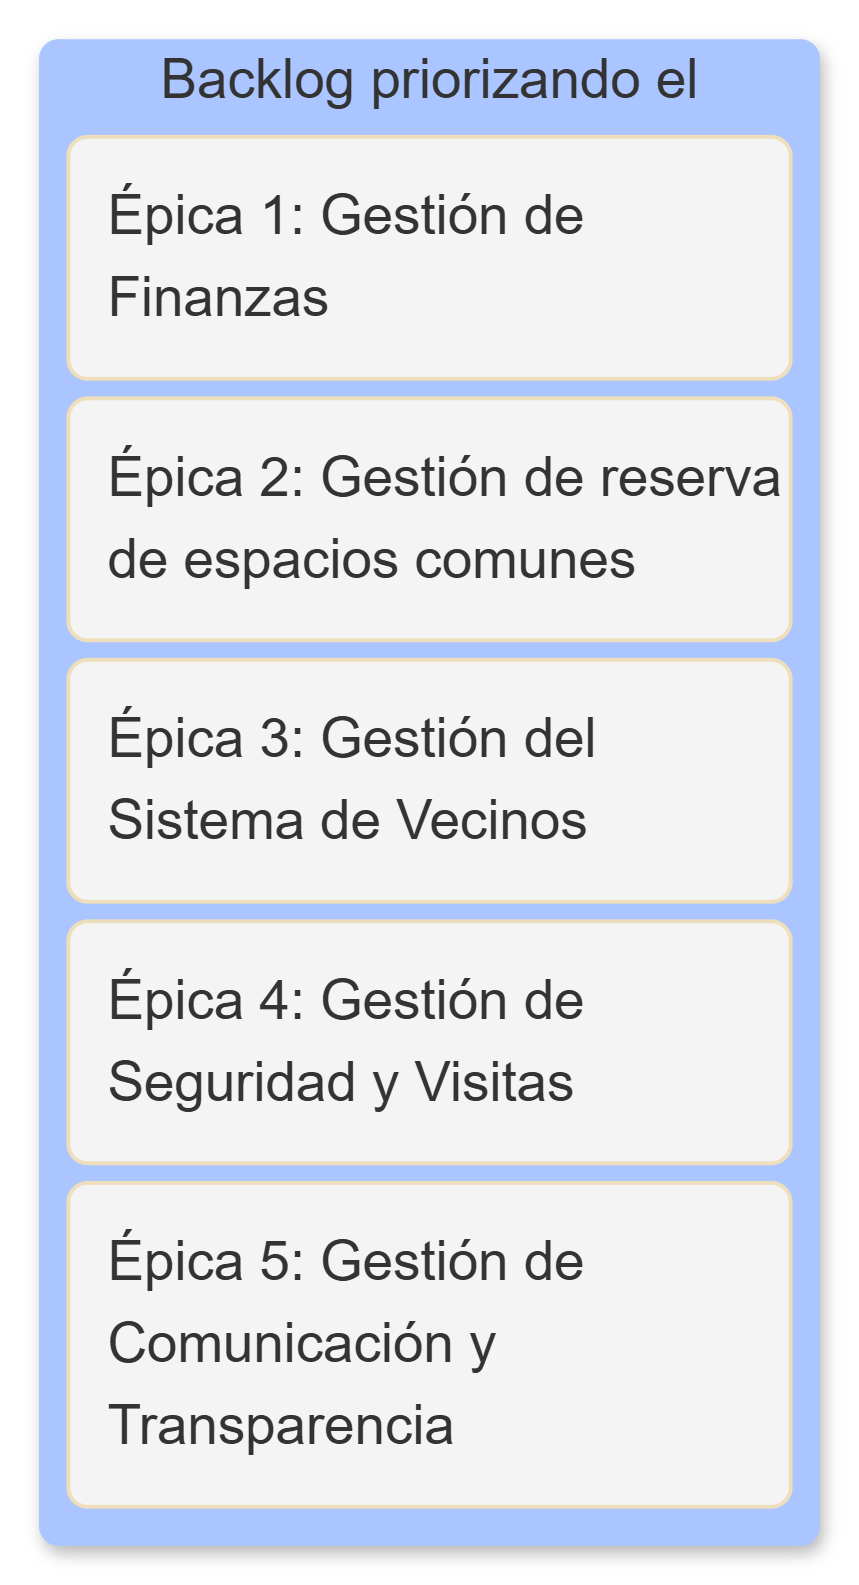
\includegraphics[width=0.313\textwidth]{figures/lista-de-backlog-con-las-epicas.png}
    \caption{Lista de BackLog con las épicas.}
\end{figure}



\textbf{Planificación de la liberación}

Tras el análisis del \textit{Product Backlog}, el Equipo Scrum ha priorizado las entregas basándose en el valor de negocio. Se determinó que el núcleo del sistema es el módulo contable, por lo que la Épica 1 (Gestión de Finanzas) conformará la primera liberación. Las entregas subsecuentes abordarán la gestión de reservas, usuarios, seguridad y comunicación.  

\textbf{Liberación 1: Gestión Financiera Base (Duración: 2 Sprints de 2 semanas)}
Para esta primera entrega, aplicamos una estricta priorización, seleccionando únicamente las Historias de Usuario (HU) críticas para el funcionamiento empírico del sistema, divididas en tres ejes:
\begin{itemize}
    \item \textbf{Estructura Base:} HU1 (Registro del Edificio) y HU2 (Configuración de Departamentos/ Alquileres). Son dependencias absolutas; sin la configuración inicial, el sistema carece de viabilidad.
    \item \textbf{Motor de Expensas (Administrador):} HU3 (Ingreso de Gastos), HU5 (Generar liquidación mensual) y HU6 (Registro manual de pagos). Permiten el registro de facturas, la generación de totales y el control de transferencias.  
    \item \textbf{Visibilidad (Inquilino/Propietario):} HU11 (Consultar mi estado de deudas), HU15 (Consultar gastos de expensa mensual) y HU13 (Pagar de deudas Online). Garantizan que el usuario final tenga claridad inmediata sobre su estado de cuenta.
\end{itemize}

Las funcionalidades secundarias de la Épica 1 (HU7 - Cálculo automático de intereses, HU10 - Notificaciones automáticas, HU14 - Subir comprobante y HU16 - Confirmar pago por transferencia) permanecerán en el \textit{Product Backlog} para iteraciones futuras, mitigando así los riesgos técnicos de esta primera entrega.  

\textbf{Liberación 2: Gestión de Espacios y Usuarios (Duración: 2 Sprints de 2 semanas)}
Esta liberación integrará las funcionalidades esenciales de dos grandes módulos para expandir el valor entregado al consorcio:
\begin{itemize}
    \item \textbf{Épica 2 (Reserva de espacios comunes):} Se implementarán la HU17 (Ver disponibilidad), HU18 (Solicitar reserva) y HU20 (Cancelar reserva), dejando el módulo operativo para los residentes.  
    \item \textbf{Épica 3 (Sistema de Inquilinos/Propietarios):} Se abordarán la HU22 (Alta de usuario), HU23 (Actualización de datos) y HU24 (Baja o desvinculación). Las tareas de gestión administrativa profunda (HU19, HU21 y HU25) se postergan para evitar comprometer los plazos y la estabilidad del incremento.
\end{itemize}

\textbf{Liberación 3: Seguridad y Transparencia (Duración: 2 Sprints de 2 semanas)}
Dado que la complejidad técnica y el esfuerzo estimado de las épicas restantes es menor, esta entrega abarca la totalidad de las funcionalidades planificadas para los módulos 4 y 5, sin representar un riesgo para el cronograma del proyecto:
\begin{itemize}
    \item \textbf{Épica 4 (Seguridad y Visitas):} HU26 (Ingreso de visita), HU27 (Recepción de paquetería) y HU28 (Confirmar retiro).  
    \item \textbf{Épica 5 (Comunicación):} HU29 (Publicar comunicado), HU30 (Consultar documentos) y HU31 (Enviar consulta a administración).
\end{itemize}
